\documentclass[12pt]{article}
\usepackage{amsmath}
\usepackage{graphicx,psfrag,epsf,subcaption}
\usepackage{enumerate}
\usepackage{natbib}
\usepackage{url} % not crucial - just used below for the URL 

%\pdfminorversion=4
% NOTE: To produce blinded version, replace "0" with "1" below.
\newcommand{\blind}{0}

% DON'T change margins - should be 1 inch all around.
\addtolength{\oddsidemargin}{-.5in}%
\addtolength{\evensidemargin}{-.5in}%
\addtolength{\textwidth}{1in}%
\addtolength{\textheight}{1.3in}%
\addtolength{\topmargin}{-.8in}%


\begin{document}

%\bibliographystyle{natbib}

\def\spacingset#1{\renewcommand{\baselinestretch}%
{#1}\small\normalsize} \spacingset{1}
\setlength{\parindent}{5ex}


%%%%%%%%%%%%%%%%%%%%%%%%%%%%%%%%%%%%%%%%%%%%%%%%%%%%%%%%%%%%%%%%%%%%%%%%%%%%%%

\if0\blind
{
  \title{\bf Matrix Explorer: A Web Application for Data Exploration}
  \author{Ivan A. Kuznetsov and Joshua T. Vogelstein\thanks{
  		The authors gratefully acknowledge \textit{please remember to list all relevant funding sources in the unblinded version}}\hspace{.2cm} \\
    Department of Biomedical Engineering, The Johns Hopkins\\
    University, Baltimore, Maryland 21218, USA}
  \maketitle
} \fi

\if1\blind
{
  \bigskip
  \bigskip
  \bigskip
  \begin{center}
    {\LARGE\bf Title}
\end{center}
  \medskip
} \fi

\bigskip
\begin{abstract}
\noindent Exploration and visualization of structured data is crucial to driving discovery across a multitude of different basic science fields. Unfortunately, oftentimes basic researchers lack the statistical knowledge to analyze their data. In this paper we describe Matrix Explorer, a novel data exploration and visualization web application. The tool allows users to upload and explore small to medium sized structured datasets. The current tool is optimized for files of size less than 1 Gb. Within Matrix Explorer we have implemented some very basic techniques which we believe are relevant to any sort of data analyses: (i) data reordering, sorting, and searching; (ii) data visualization via heatmap , scatter/box/violin plots, marginal distributions, and 2D embedding; (iii) data exploration via k-means clustering, dendrogram, correlation and covariance matrix computation, and outlier detection. We validated Matrix Explorer by showing that it produces reasonable results for the iris flower dataset. We then used Matrix Explorer to analyze a novel SPECT image dataset.
\end{abstract}

\noindent%
{\it Keywords:}  3 to 6 keywords, that do not appear in the title
\vfill

\newpage
\spacingset{1.45} % DON'T change the spacing!
\section{Introduction}
\label{sec:intro}

The past decade has seen an explosion in scientists' ability to collect huge quantities of data and a simultaneous growth in the necessary computational power and statistical framework to process said data. Unfortunately, despite a multitude of attempts [CITE], exploratory analysis of novel datasets remains more of an art than an exact science, requiring a thorough understanding of statistical science to perform properly. The result of this phenomenon is that the a large quantity of collected data, especially in the basic sciences, is rather poorly analyzed, undoubtedly decreasing the pace of new discoveries.

What is then required is a framework within which users with minimal statistical knowledge can explore their data. To the best to of our knowledge, such a tool does not yet exist. The R, MATLAB, and Python languages and associated toolboxes and packages still require users to have a non-negligable understanding of underlying methods in order to conduct proper data analysis. Other attempts at decreasing the barrier to entry for quality exploratory data analysis such as GGobi and ViSta, as described in \cite{swayne2003ggobi} and \cite{valero2011using} respectively, have not resolved the issue, requiring a significant learning curve to utilize.

In this paper we describe Matrix Explorer (MX), a novel data exploration web application built via the R Shiny package. Within MX we have included the techniques which we deem nest practice whenever starting a new exploratory analysis task. MX provides users with minimal knowledge of statistics the tools necessary to conduct a basic characterization of their data.

\section{Methods \& Validation}
\label{sec:meth}

MX is implemented via the R Shiny package, which allows for the construction of interactive web applications which use R as their backend. The Shiny server is hosted on a Docker instance. The functionality of MX is divided into several different submodules, organized as tabs in the web application, which we  describe in depth below. Furthermore, we provide visualizations and validation of the ability of MX to allow for basic data analysis by provided by exploring the iris flower dataset. 

The iris dataset is composed of 50 samples from each of three types of iris flower (\textit{setosa}, \textit{virginica}, and \textit{versicolor}). For each sample four features are measured, specifically the length and width of the sepal and petals. For the purposes of the validation, we added a fifth feature column which gives the class label of each sample. We now seek the show that MX can detect that the samples should cluster into three distinct groups.

\subsection{Data Upload \& Selection}
\label{subsec:SubSecUpload}

Upon opening the application, the user is first prompted to upload a dataset. Note that MX assumes that rows in the dataset represent samples and columns represent features. Once uploading is complete, the user may then select the rows and columns that he or she wishes to analyze and also flag a specific column as a class label column. The current implementation accepts comma separated variable (CSV) files and is optimized for sizes below 1 gigabyte. Hence, we converted our iris dataset to csv format and uploaded it to MX using the interface.

\subsection{Heatmap \& Dendrogram}
\label{subsec:SubSecHeatmap}

\begin{figure}[t!]
	\centering
	\begin{subfigure}[b]{0.8\textwidth}
		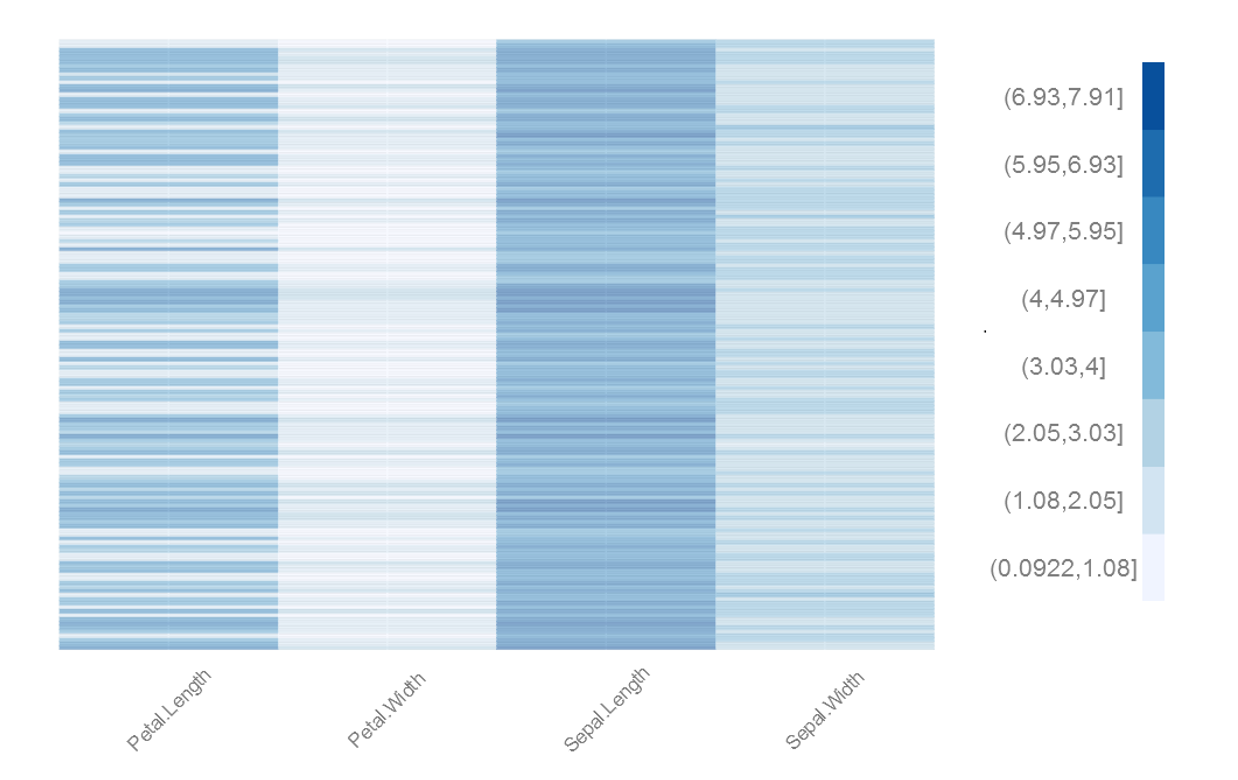
\includegraphics[width=\textwidth]{Figures/Iris/HeatmapRawnodendro.png}
		\subcaption{}
		\label{fig:FigHeatmapRawnodendro}
	\end{subfigure}
	\begin{subfigure}[b]{0.8\textwidth}
		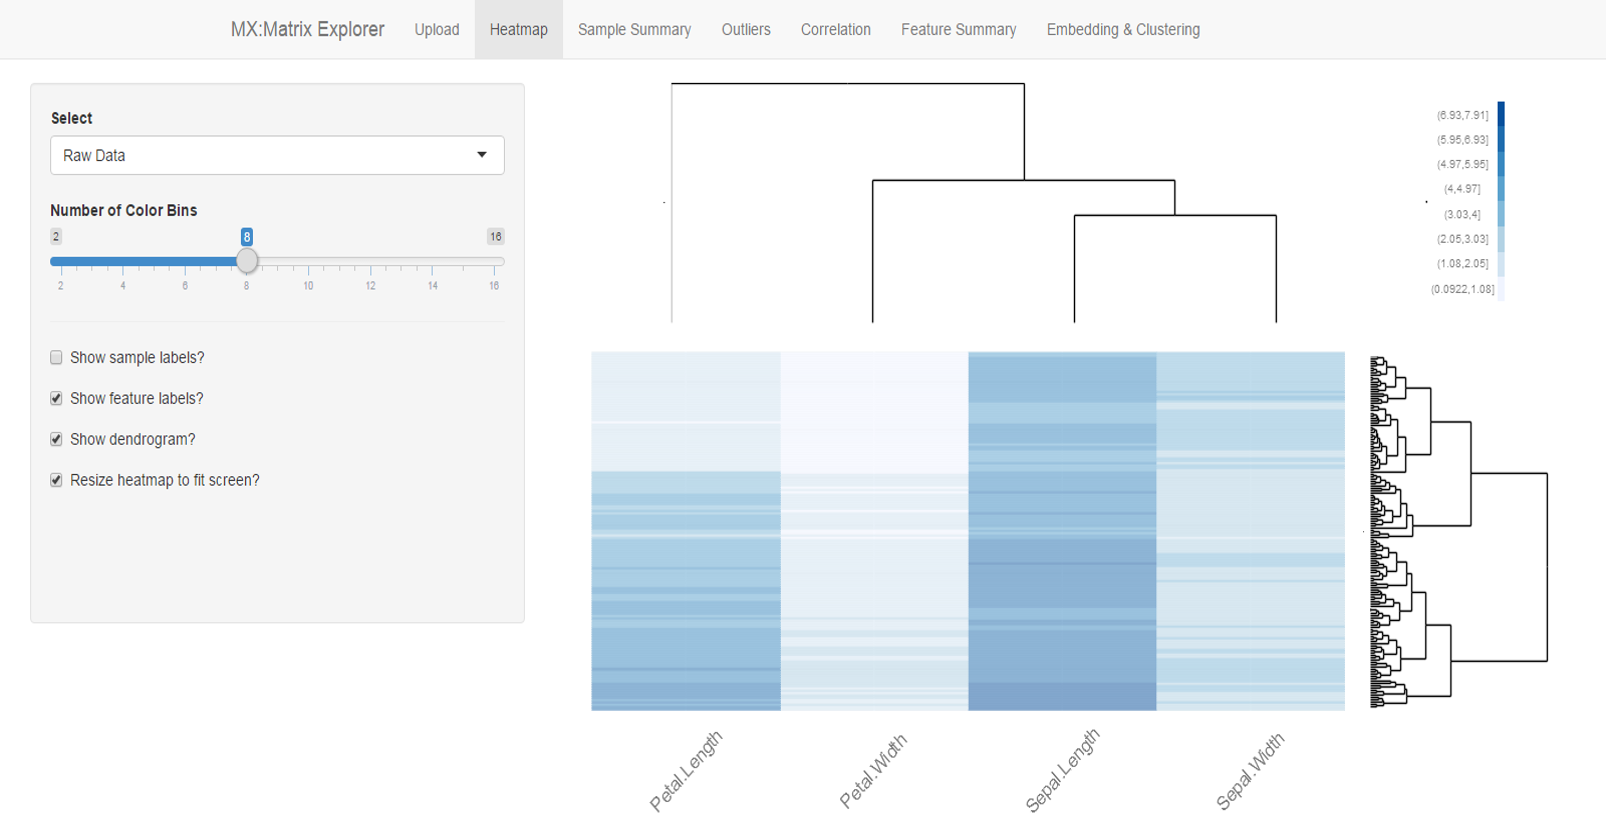
\includegraphics[width=\textwidth]{Figures/Iris/HeatmapRaw.png}
		\subcaption{}
		\label{fig:FigHeatmapRaw}
	\end{subfigure}
	\caption{Heatmap of iris dataset for various visualization options. Sample labels are not shown. (a) Heatmap of raw data. Note that there is no evidence for the existence of clusters. (b) Heatmap of raw data with dendrogram and associated row and column sorting. The existence of at least two clusters is clear.}
	\label{fig:FigHeatmap}
\end{figure}

A heatmap provides the most direct way of visualizing the data, besides simple looking at it as a data table. However, oftentimes clear trends in the data are obscured on a heatmap because of varying ranges amongst features. Normalization resolves this issue.

MX allows users to construct a heatmap of their data and gives them the option to normalize it via conversion to z-scores, quantiles, or ranks. Furthermore, for datasets with less than 100 rows and columns, MX uses hierarchical clustering to compute a dendrogram of the dataset and display it, reordering the columns and rows as necessary. 

Some of these capabilities are demonstrated in Figure~\ref{fig:FigHeatmap}. 

\subsection{Sample Summary}
\label{subsec:SubSecSample}

\begin{figure}[t!]
	\centering
	\begin{subfigure}[b]{0.8\textwidth}
		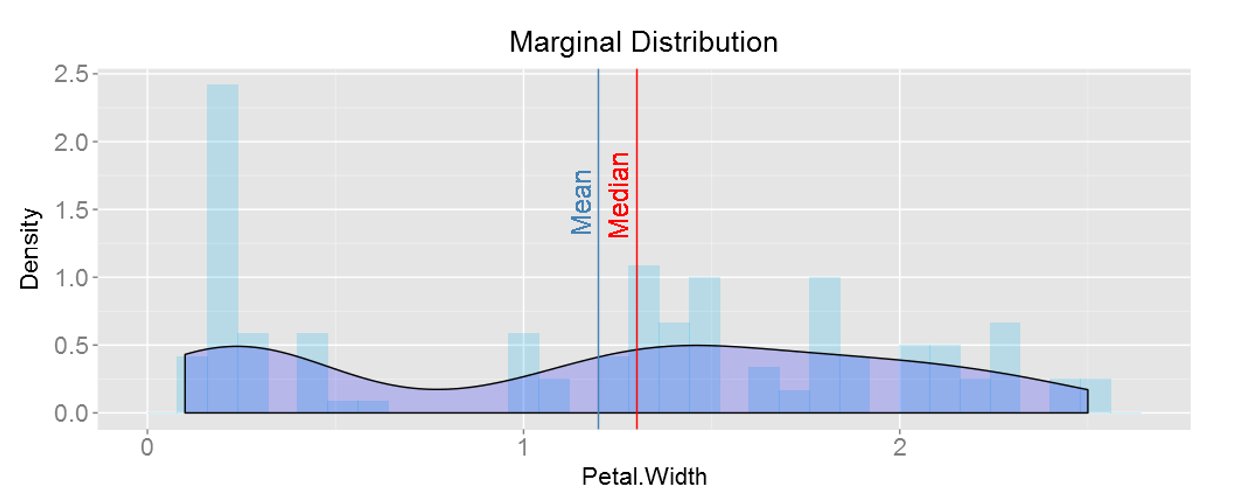
\includegraphics[width=\textwidth]{Figures/Iris/MarginalPetalWidthnocond.png}
		\subcaption{}
		\label{fig:FigMarginalNoCond}
	\end{subfigure}
	\begin{subfigure}[b]{0.8\textwidth}
		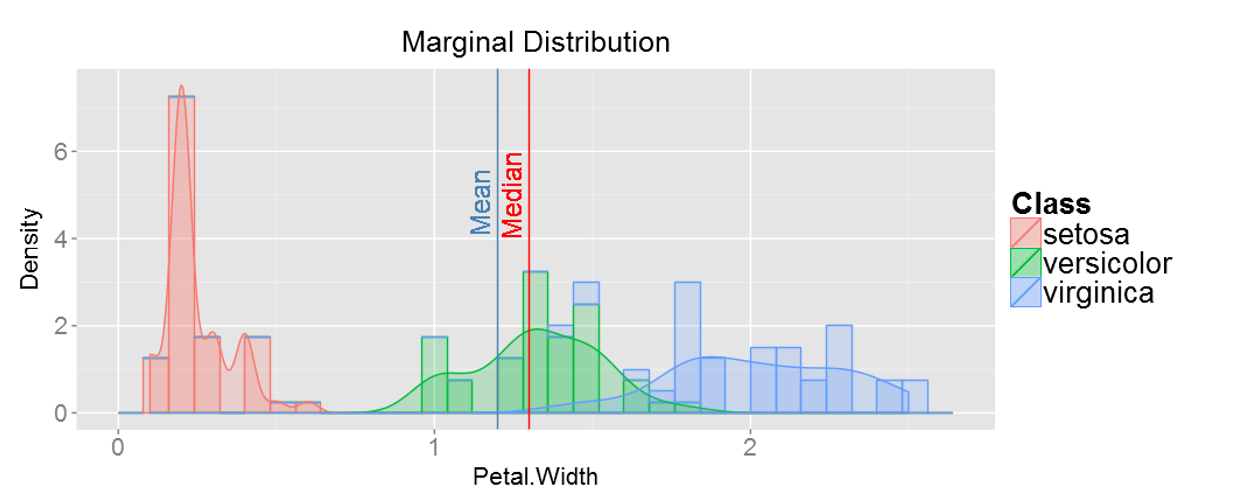
\includegraphics[width=\textwidth]{Figures/Iris/MarginalPetalWidth.png}
		\subcaption{}
		\label{fig:FigMarginal}
	\end{subfigure}
	\caption{Marginal of the petal width feature of the iris dataset. (a) Histogram and kernel density estimate of the samples without conditioning on class. Note that it is unclear whether the distribution is multi-modal. (b) Histogram and kernel density estimate of the samples after conditioning on class. It is now clear that the marginal distribution is tri-modal.}
	\label{fig:FigSample}
\end{figure}

MX allows users to visualize the marginal distributions of the individual feature columns. MX can generate either a histogram, a kernel density estimate, or a overlay of both. The mean and median is indicated on the plot. Additionally, if the user labeled a feature as a class label column, he or she has the option of conditioning the marginal on classes. This latter feature is incredibly useful for feature selection and determining the separability of the data based on class label within the feature space. This capability is demonstrated in Figure~\ref{fig:FigSample}. 

The robust Mahalanobis distances, shown in  Figure~\ref{fig:IrisOutliers}, indicate that the first 50 samples are far away from the last 100 samples. This is expected, as these first 50 samples belong to the \textit{Iris setosa} class, while the last 100 belong to the \textit{Iris virginica} and \textit{Iris versicolor} class. Interestingly, the outlier analysis does not indicate a difference in distance between the samples from the \textit{Iris virginica} and \textit{Iris versicolor} class. Two-dimensional embedding via both PCA and tSNE visually separate the data into three distinct groups. The results with PCA are shown in Figure~\ref{fig:IrisEmbedding} after k-means with \textit{k = 3}.

Therefore, we have shown that MX provides the ability to explore the iris dataset, helps construct visualizations of the distribution of the data, and acts a sa basic tool to help in the initial characterization of a dataset.

\subsection{Outliers}
\label{subsec:SubSecOutliers}

\begin{figure}[t!]
	\centering
	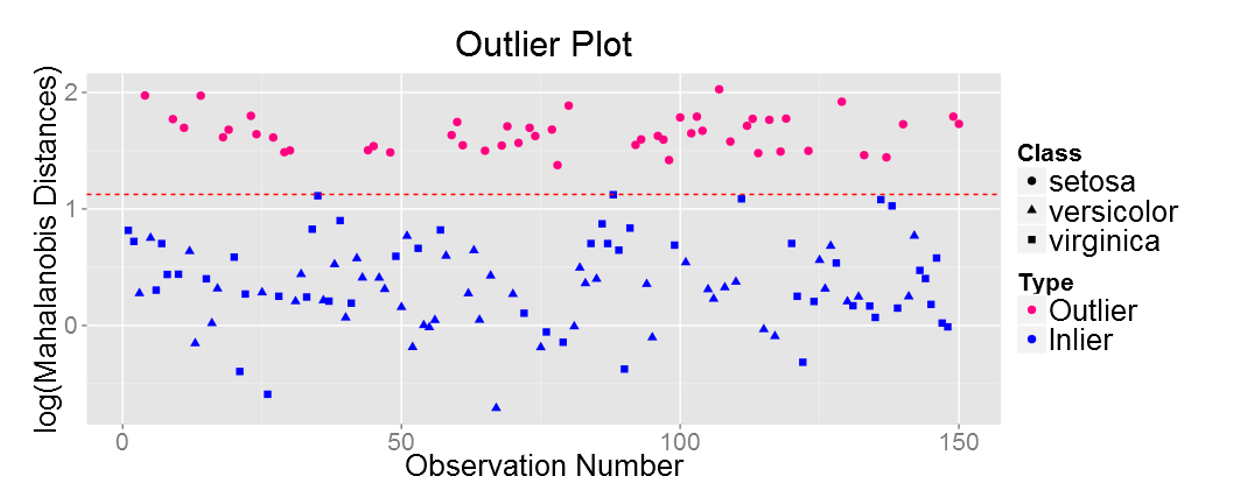
\includegraphics[width=0.8\textwidth]{Figures/Iris/OutliersIris.png}
	\caption{Robust Mahalanobis distances with choice of alpha cut-off value to reject samples as outliers on the iris dataset. Note that 51 of the 150 samples are flagged as outliers. Such as large number of outliers usually indicates the existence of samples which belong to a separate group than the rest of the data. As a matter of fact, 50 of these 51 samples belong to the \textit{Iris setosa} class, which is apparently quite far from the samples which belong to the \textit{Iris virginica} and \textit{Iris versicolor} classes.}
	\label{fig:FigOutliers}
\end{figure}

In order to determine outliers it is necessary to first establish a distance metric to determine how far away a specific sample is from other samples. In this case, robust Mahalanobis distances were used, as described in \cite{hubert2008high}. Briefly, a robust estimate of the sample mean and covariance was first approximated via either: 1) the fast minimum covariance determinant algorithm (FAST-MCD) as described in \cite{rousseeuw1999fast} or 2) the Orthogonalized Gnanadesikan-Kettenring algorithm (OGK) as described in \cite{maronna2002robust}. Specifically, FAST-MCD was used for low dimensional datasets, while OGK was used for high dimensional datasets to the fact that FAST-MCD scales poorly with increasing dimensionality. Next, using these robust measures, the Mahalanobis distance of each sample was computed. As explained by \cite{hardin2012distribution} [FIND BETTER CITATION?], the squares of the robust Mahalanobis distances are approximately distributed $\chi^2_n$, where $n$ is the dimensionality of the dataset . It is then possible to define a alpha value above which to reject a sample as an outlier. 

MX allows the user to set this alpha value and graphically displays the robust Mahalnobis distances and resulting threshold. This is shown in Figure~\ref{fig:FigOutliers}.

\subsection{Correlation}
\label{subsec:SubSecCorrelation}

Knowledge of which features are correlated is highly relevant besides assumption checking and feature selection in building classifiers. Similarly, they may aid in providing an intuitive understanding of the underlying patterns within the data. For example, in gene expression datasets these correlations may suggest the biological importance of various genetic markers [ANOTHER CITATION]. To see an example of when this is useful, we refer the reader to \cite{shi2012unsupervised} [BETTER CITATION].

MX computes the Pearson's correlation amongst features and displays it to the user. To better understand the interactions and distributions of features, MX can also compute the euclidean distance between features. To account for scaling effects, users have the option of pre-processing the data via conversion to z-scores, quantiles, or ranks. Furthermore, users can remove the outliers detected in the outlier tab from the data before computing the metrics. 

\subsection{Feature Summary}
\label{subsec:SubSecFeature}

\begin{figure}
	\centering
	\begin{subfigure}[b]{0.8\textwidth}
		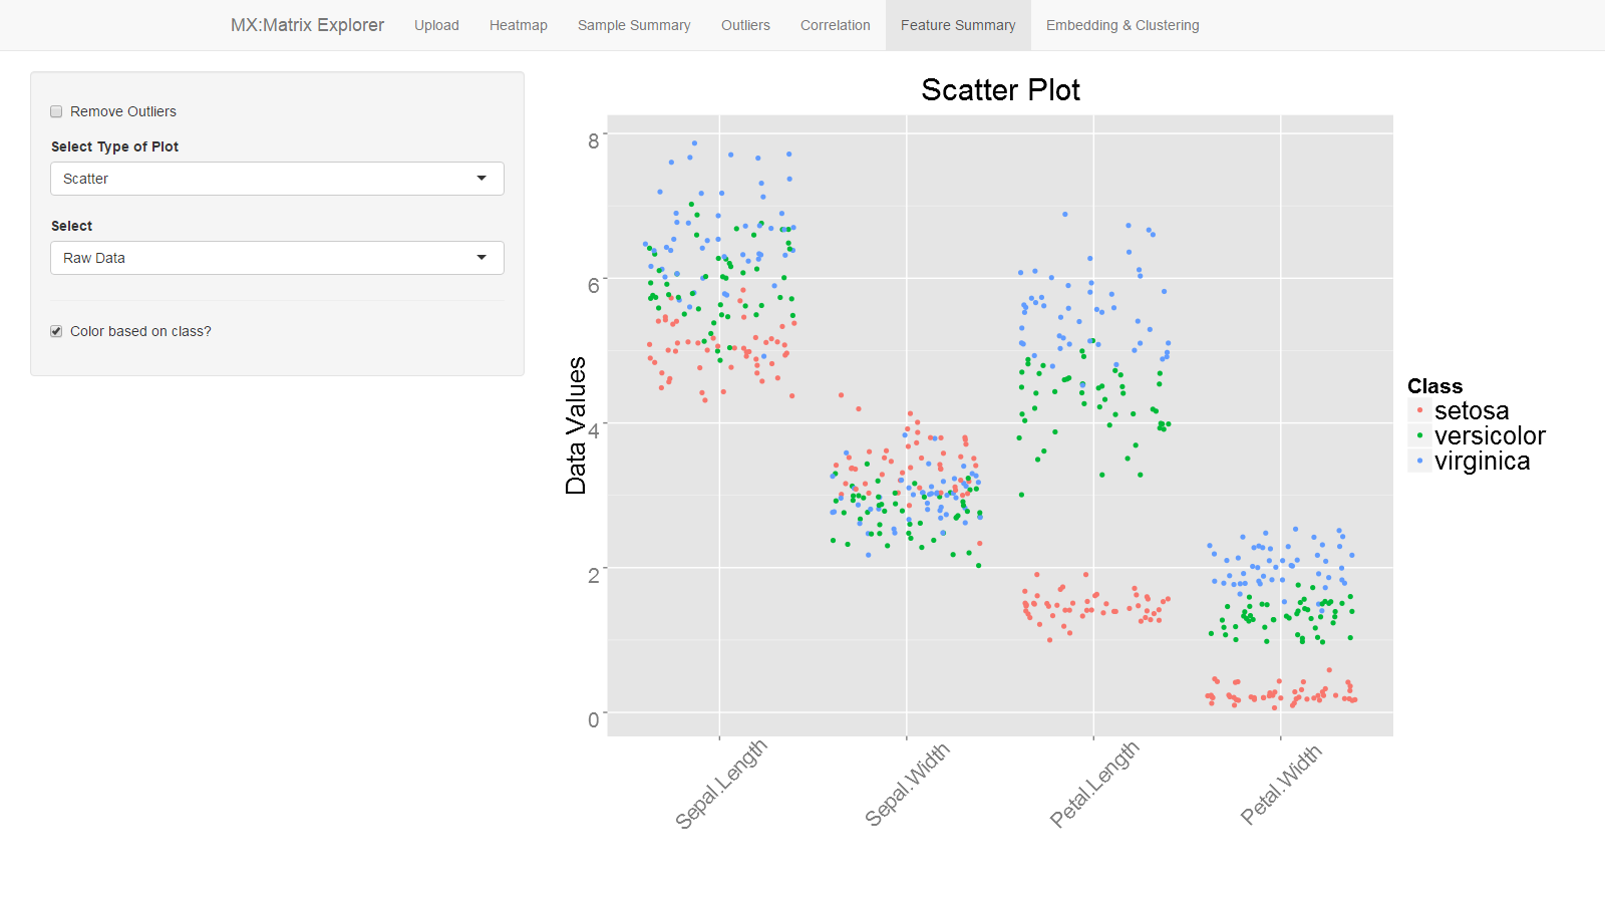
\includegraphics[width=\textwidth]{Figures/Iris/ScatterColor_Raw.png}
		\subcaption{}
		\label{fig:FigScatter}
	\end{subfigure}
	\begin{subfigure}[b]{0.8\textwidth}
		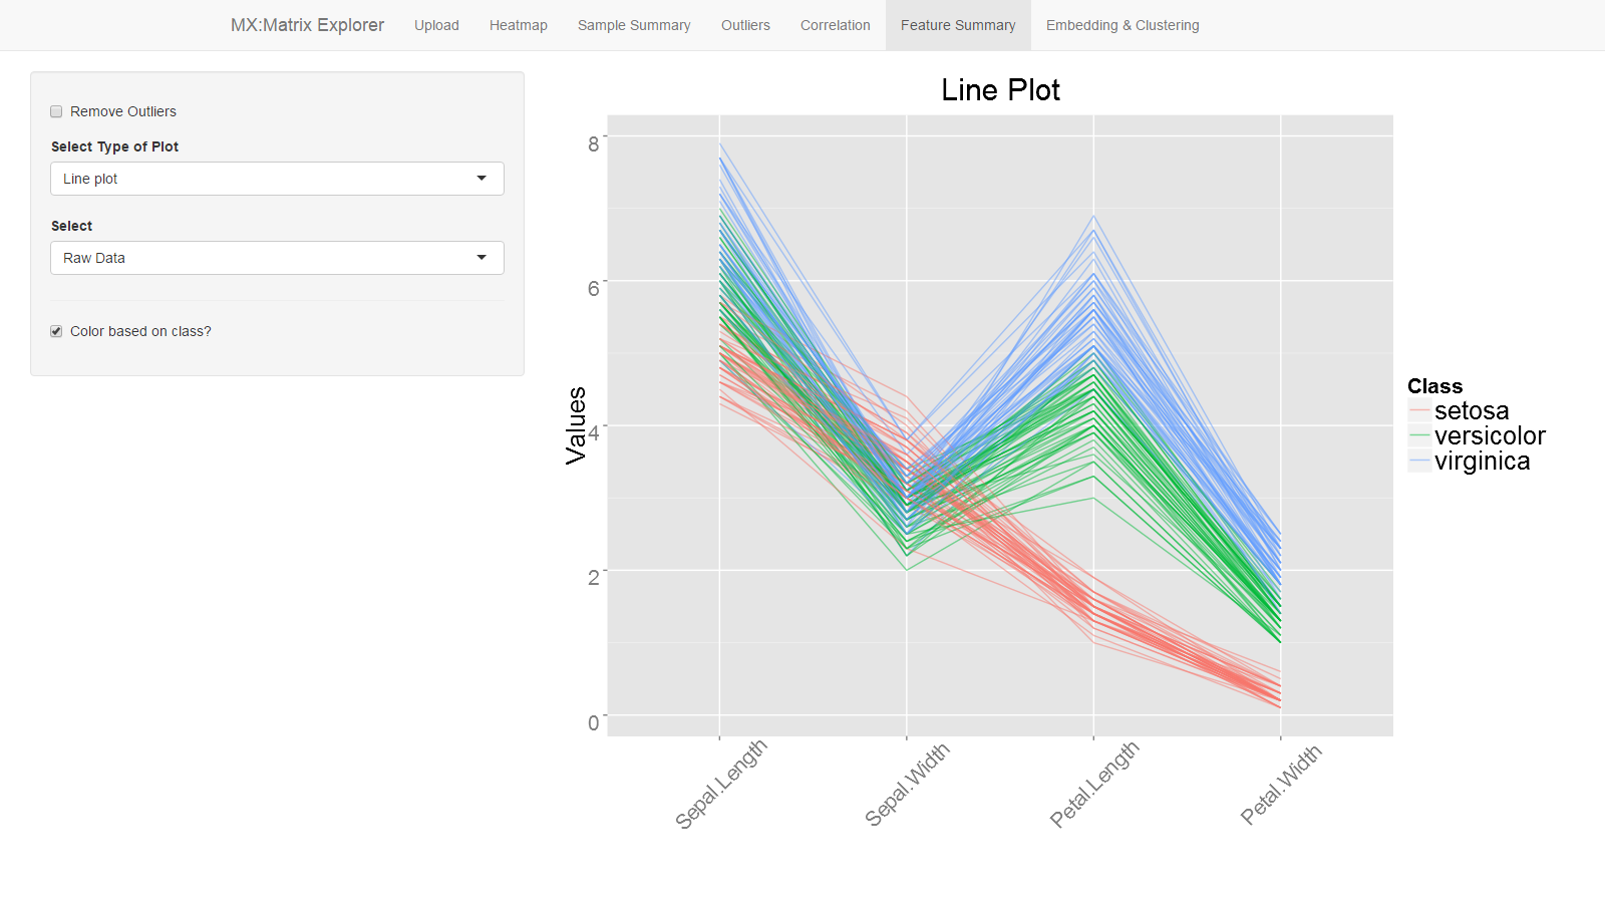
\includegraphics[width=\textwidth]{Figures/Iris/LineColor_Raw.png}
		\subcaption{}
		\label{fig:FigLine}
	\end{subfigure}
	\caption{Visualization of the samples across all the features in the iris dataset. (a) Jittered scatter plot of the sample values across the features and colored based on class label. Note that the multi-modal nature of the petal width and petal length marginal distributions is clear. It is also apparent that the samples from the \textit{Iris setosa} class are very different from the samples from the other two classes. (b) Line plot showing the behavior of individual samples across the features. Each line represents the values a sample takes on at the corresponding feature. Visually, it is clear how differently the samples from the \textit{Iris setosa} class behave compared to samples from the other classes. Note also that we can now visually see the absence of actual outliers.}
	\label{fig:FigFeature}
\end{figure}

MX allows users to visualize the marginal distributions of all the features on the same plot. This is done via a jittered scatter plot, vector of sample means with standard error bars, a box plot, and a violin plot. In order to ensure that outliers do not skew the visualizations, users have te options of removing outliers detected in the outlier tab from the dataset before generating the plots. These capabilities are shown in  Figure~\ref{fig:FigFeature}.

\subsection{Embedding \& Clustering}
\label{subsec:SubSecEmbedding}

\begin{figure}[t!]
	\centering
	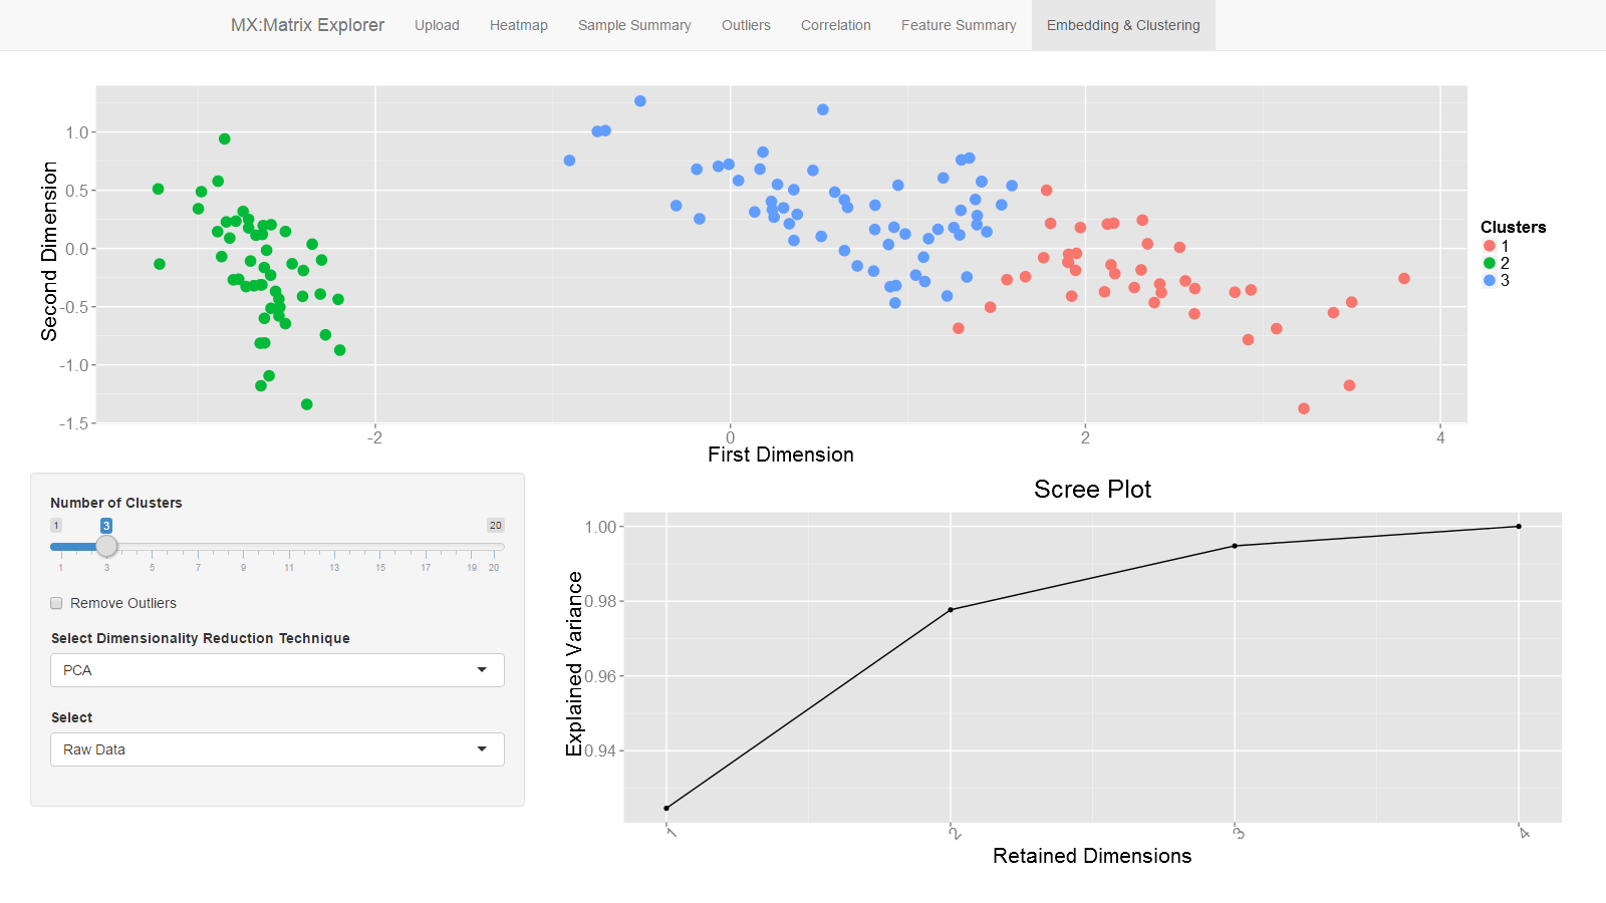
\includegraphics[width=0.8\textwidth]{Figures/Iris/Embed_Raw.png}
	\caption{Two-dimensional embedding of samples using PCA followed by coloring using labels given by k-means clustering with \textit{k = 3}. Samples clearly group into 2-3 clusters.}
	\label{fig:FigEmbedding}
\end{figure}

One of the most intuitive ways of visualizing bivariate data is a scatter plot. Although this is not directly possible for data with more than two dimensions, various dimensionality reduction techniques can be used to embed the data within a two-dimensional coordinate system for simple examination of general structure and clustering. Dimensionality reduction techniques can be further reduced into linear and non-linear methods, both of which have their own unique advantages and disadvantages. For an overview of techniques we refer the reader to \cite{van2009dimensionality}. Within MX we have implemented one linear method, principle component analysis (PCA), and one non-linear method, t-distributed stochastic neighbor embedding (tSNE). For a thorough description of how tSNE works, see \cite{van2008visualizing}.

Note that PCA is extremely sensitive to (1) the scaling of the data and to the (2) presence of outliers.  Hence, to overcome (1), MX allows users to normalize the feature columns by converting either to z-scores, quantiles, or ranks. Note that conversion to quantiles or ranks also decreases the sensitivity of the embedding to outliers, hence aiding in overcoming (2). MX also allows users to resolve (2) more directly by giving them the option to remove the outliers detected in the outliers tab before generating the visualization. In order to inform the users of how much information was lost by embedding the data set into two dimensions, MX also displays a scree plot, which indicates the percentage of retained variance after PCA. The described properties can be seen in Figure~\ref{fig:FigEmbedding}.

\section{Results}
\label{sec:res}
We next used MX to explore a previously unanalyzed dataset.

\section{Conclusion}
\label{sec:conc}

We have created MX, a web application driven by the R Shiny package, which allows for basic data exploration and visualization of small to medium sized datasets. Within MX, we have included the tools whose usage we believe to be best practice whenever exploring a new dataset. We have validated the functionality of MX by demonstrating its capability to characterize the iris flower dataset and determine the presence of three different classes. We have then used MX to explore a previously uncharacterized dataset, a collection of SPECT images from over 5000 patients.

Although the implemented algorithms may seem simplistic to those with a statistical background, they are highly relevant to MXs target user base: scientists with minimal knowledge of statistical techniques.

\section{Acknowledgments}
\label{sec:ack}
We would like the thank XXX for helpful discussions.

\bigskip
\begin{center}
{\large\bf SUPPLEMENTARY MATERIAL}
\end{center}

Probably stuff from above will get moved here.

\bibliographystyle{Chicago}

\bibliography{BibliographyMX}
\end{document}
